\documentclass[a4paper,11pt]{article}

% set up sensible margins (same as for cssethesis)
\usepackage[paper=a4paper,left=30mm,width=150mm,top=25mm,bottom=25mm]{geometry} 
\usepackage{natbib} % Use the natbib bibliography and citation package
\usepackage{setspace} % This is used in the title page
\usepackage{graphicx} % This is used to load the crest in the title page
\usepackage{tikz} %Finite state automata
\usepackage{subfig}
\usepackage{amsmath}
\renewcommand{\bibsection}{\section{References}}
%\usepackage{hyperref}
%\hypersetup{
%   colorlinks,
%    citecolor=black,
%    filecolor=black,
%    linkcolor=black,
%    urlcolor=black
%}

\usepackage[singlelinecheck=false]{caption}
\usetikzlibrary{arrows,automata}

\begin{document}

% Set up a title page
\thispagestyle{empty} % no page number on very first page
% Use roman numerals for page numbers initially
\renewcommand{\thepage}{\roman{page}}

\begin{spacing}{1.5}
\begin{center}
{\Large \bfseries
Clayton School of Information Technology\\
Monash University}

\vspace*{30mm}


\includegraphics[width=5cm]{MonashCrest}

\vspace*{15mm}

{\large \bfseries
Research Proposal --- Semester 1, 2014
}

\vspace*{10mm}

{\LARGE \bfseries
Simulated Evolution of Non-Regular Strategies for Repeated Games
}

\vspace*{20mm}

{\large \bfseries
Bradon Thomas Hall \\22051635\\
\today

\vspace*{20mm}

Supervisor: \parbox[t]{50mm}{Julian Garcia}
}

\end{center}
\end{spacing}

\newpage

\tableofcontents

\newpage
% Now reset page number counter,and switch to arabic numerals for remaining
% page numbers 
\setcounter{page}{1}
\renewcommand{\thepage}{\arabic{page}}
%Create a research proposal (approximately 3000 words) that clearly identifies the 
%agreed research topic, identifies the problem being studied, and justifies the aims 
%and significance of the project. The proposal should include a discussion of the 
%research context and background, the proposed methodology, the research design 
%and deliverables. 
%The proposal should also be presented professionally with a standard of written 
%expression appropriate to research publications in the field. 
\section{Introduction}
Cooperation, working together for a common goal, is a widely observed behaviour. 
Many animal species, from micro-organisms to social animals, such as humans, exhibit some cooperative behaviour. 
How did this evolve, and why do exploitative variants not disrupt the behaviour? 
Study of the evolution of cooperative strategies provides insight into problems in biology or any field where competition is relevant, for example economics and the social sciences \citep{Axelrod1997}. 

How cooperation evolves in a group of individuals is not fully understood. 
Individually, exploiting cooperative behaviour gives an individual an advantage. 
But if there is no one to exploit, this strategy is not advantageous. 
Everyone cooperating gives a better outcome, but no individual has an immediate incentive to switch. 
Evolutionary Game Theory is useful for predicting the outcome of evolution where fitness of individuals is related to behaviour of other individuals of that population \citep{maynard-smith:book:1982}. 
Computational science can be used to investigate Evolutionary Game Theory, evolving populations in various simulated environments and analysing the outcome \citep{fogel1993evolving}. 

\citet{nowak:Science:2006} discussed several mechanisms for the evolution of cooperation. 
Kin selection, when cooperation with related members increases fitness of a member who shares genes. 
Direct reciprocity is another mechanism, which can be summarised as ``you scratch my back, I'll scratch yours''; this can be studied with repeated games. 
Indirect reciprocity follows, where other members of the population reward cooperators; where the choice to cooperate is influenced by the opponent's reputation. 
Nowak also discusses Network Reciprocity, where networks of cooperating members forms. 
Finally, group selection, where success of groups of individuals and success of individuals themselves is important. 
Several of these examples (particularly kin and group selection) are various forms of population structure, which will be studied in the project. 

This project aims to investigate the evolution of cooperation in repeated games, and how the computational capability of agents in the model effects the evolution of cooperation. 
A repeated version of a simple game called the Prisoner's Dilemma will be used to simulate evolution in a competitive environment with a population of players. 
The strategies players use are randomly mutated (a Genetic Programming method), and ones that perform well in the game selected for survival- this is inspired by biologic evolution. 
This technique has been widely used to investigate behavioural biology with game theory, but richer models are necessary to improve applicability \citep{McNamara2013}. 
This work intends to contribute towards that goal. 

Strategies in repeated games can be studied via a variety of means; analytic evaluation of strategies from game theoretic approaches is one method. 
This method is particularly powerful for the study of simple strategies, or small sets of strategies. 
Computational methods provide a means to study a wider variety of strategies \citep{fogel1993evolving}. 
Using a representation that allows strategies to be mutated by a simple stochastic process allows the simulation to explore a set of strategies without manual input. 
For example, in a Finite State Automata implementation states and state transitions can be added and removed to form a new strategy. 
Strategies are removed from the population as a result of the outcome of the repeated game- the fitness of the strategy determines its survival. 
The results of simulations can be used to inform analysis of the these strategies, and analysis of how these strategies evolve.

Cooperation in repeated games was investigated by \citet{van-veelen:PNAS:2012}. 
They looked into two models of cooperation- direct reciprocity and population structure- and the relation between them, using Finite State Automata to represent strategies in the simulation. 
In this project more computationally powerful methods of representing strategies will be tested and the results compared to previous research.

The results may assist in general by further revealing the limitations or usefulness of simple evolutionary models. 
In particular, recent research has provided models with cooperation resembling human behavior more closely, and this project may help to refine, extend, or find limitations of this model.
%\pagebreak[4]
\section{Research Context}
\subsection{The Prisoner's Dilemma}
The Prisoner's Dilemma is a simple model that has been widely used to study cooperation in repeated games \citep{Axelrod1997}. 
In the one-shot version of the Prisoner's Dilemma, cooperation is not the expected outcome. 
In this game, two players play a single game, choosing between two options; cooperate or defect. 
Players choose simultaneously, and have no information on the opponents choice before their own decision is made. 
If they both cooperate they receive a score of R (Reward for cooperation). 
If they both defect, they receive a score of P (Punishment for defection). 
If one player defects, and their opponent cooperates, the defector is rewarded with T (Temptation to defect). 
If a player cooperates, and their opponent defects, the cooperator receives a payoff of S (Sucker's punishment). 
The hierarchy of payoffs goes $T>R>P>S$. Table \ref{table:payoffs} shows the payoff matrix for the Prisoner's Dilemma. 
\begin{table}[h]\centering
\captionsetup{justification=centering}
\begin{tabular}{|l|c|c|}
\hline
 & Cooperate & Defect\\
\hline
Cooperate & R & S\\
\hline
Defect & T  & P \\
\hline
\end{tabular}
\caption{Payoff Matrix for the Prisoner's Dilemma.\\ Player choice left, opponent choice top.}
\label{table:payoffs}
\end{table}

Assuming both players are aware of the payoff table and both players act to maximise their personal payoff, defection is the strategy both players choose. 
If the opponent defects, the best move is to defect too to avoid paying the cost. 
If the opponent cooperates, the best move is to defect to avoid the cost, and gain the benefit. 
That is, the player can only lessen the payoff by cooperating- this is a Nash equilibrium. 
The dilemma arises from the fact that mutual cooperation would be a better result for both players than the equilibrium of mutual defection. 
This game captures the essence of the problem of cooperation. %Couldnt improve on JGs wording
%\pagebreak[4]
\subsection{Assortment}
In order for cooperative behaviour to compete successfully with non-cooperative behaviour, some advantage needs to exist. 
The evolution of cooperative behaviour from a population of randomly interacting members is problematic \citep{axelrod:Science:1981}. 

A solution in order to allow evolution of cooperative behaviour is to add structure to the population. 
This also better reflects most situations that can be modelled with evolutionary simulations \citep{eshel:PNAS:1982}. 
In nature, interaction between members of a population is not likely to be randomly distributed; interaction is more likely between kin, or social peers. 
Structure can be added by changing the probability of interactions- a subset of a population is more likely to interact with that subset. 

The expected payoff for a strategy in both a structured and unstructured environment can be found analytically \citep{van-veelen:PNAS:2012}. 
Consider a strategy space consisting of only always defect and always cooperate (ALLD, ALLC). 
The potential payoff ($\Pi$) for each strategy can be calculated by the probability of meeting an ALLC opponent times the payoff in that instance plus the probability of meeting an ALLD opponent times the payoff in that instance. Where $N_{TYPE}$ is the number of a type in a population, and $N_{TOTAL}$ is the total population size ($N_{TOTAL}=N_{ALLC}+ N_{ALLD}$), the payoffs are:
\begin{align*}
\Pi_{ALLC}&=\frac{N_{ALLC}-1}{N_{TOTAL}-1} \cdot (R) + \frac{N_{ALLD}}{N_{TOTAL}-1}\cdot ({S})\\
\Pi_{ALLD}&=\frac{N_{ALLC}}{N_{TOTAL}-1} \cdot (T) + \frac{N_{ALLD}-1}{N_{TOTAL}-1}\cdot ({P})
\end{align*}

In the case of an unstructured population, since $T>R$ and $P>S$, $\Pi_D$ always has a better payoff (excluding the case when $N_{ALLD}=0$). 
Instead take the case when the population is structured, and chance of meeting an alike player is r (structure parameter):
\begin{align*}
\Pi^{(r)}_{ALLC}&=(1-r)\Pi_{ALLC}+ rR\\
\Pi^{(r)}_{ALLD}&=(1-r)\Pi_{ALLD}+ rP
\end{align*}

Sufficiently higher probability of meeting an alike player allows cooperativity to have the greater payoff. 
Trivially, if probability of meeting like is 1, $\Pi^{(S)}_{ALLC}=R>\Pi^{(S)}_{ALLD}=P$, so cooperation has higher fitness.  
Substitution of values shows it holds for other cases. 
For example, if T=3, R=2, P=1, S=0, and the population is 50 ALLC and 50 ALLD:
\begin{align*}
\Pi^{(S)}_{ALLC}&=(1-r)(2\frac{49}{99})+r*2=\frac{98}{99}+\frac{198}{99}r-\frac{98}{99}r=\frac{1}{99}(98+100r)\\
\Pi^{(S)}_{ALLD}&=(1-r)(3*\frac{50}{99} + \frac{49}{99})+ r*1=\frac{199}{99}-\frac{199}{99}r+\frac{99}{99}r=\frac{1}{99}(199-100r)
\end{align*}
So ALLC has higher fitness if $r>101/200$. These cases demonstrate that structure can benefit cooperation. 
Next, repetition of games needs to be accounted for. 
%\pagebreak[4]
\subsection{Direct Reciprocity}
When the Prisoner's Dilemma is played multiple times, all parties defecting is no longer the only successful strategy, even without structure. 
For the repeated Prisoner's Dilemma, the number of games played is not known by players in advance. 
If both players knew how many rounds were to be played, the best move in the last round is defection. 
The same logic causes the second last round to be a defection, and the problem reduces to the Nash equilibrium of the one-shot version. 
A way to accomplish having an unknown number of rounds is to make future encounters probabilistic, the chance of another encounter between two players is the continuation probability $\delta$.

\citet{garcia:PLoSOne:2012} calculate the payoff for strategy A from repeated games with strategy B as
\begin{equation}
\label{eqn:repeatedPayoff}
\Pi_{AB}=(1-\delta)\sum^{\infty}_{t=0} \delta^i\pi^i_{AB}
\end{equation}
where $\delta$ is the continuation probability, and $\pi^i$ is the payoff from the $i$th round. 
The sum represents the diminishing likelihood of another game between the two players. 
The term $(1-\delta)$ is for convenience, normalising the payoffs.
 
Two simple strategies possible in the repeated version are Tit-For-Tat (TFT) and Suspicious Tit-For-Tat (STFT). 
Tit-For-Tat starts cooperating on the first round, then reciprocates the opponents last move. 
Suspicious Tit-For-Tat defects on the first round, then reciprocates the opponents last move. 
If ALLC plays TFT, in all rounds they are cooperative.  
If TFT plays STFT they alternate defect and cooperate (Figure \ref{table:reciprocity}). 
This behaviour is an example from another model for the evolution of cooperation; direct reciprocity. 

\begin{figure}[h]
\centering
\captionsetup{justification=centering}
\begin{tabular}{|l|c|c|c|c|}
\hline
TFT & C & D & D&...\\
\hline
ALLD & D & D &D&...\\
\hline
\end{tabular}\hfill
\begin{tabular}{|l|c|c|c|c|c|}
\hline
TFT & C & D&C&...\\
\hline
STFT & D & C&D&...\\
\hline
\end{tabular}\hfill
\begin{tabular}{|l|c|c|c|c|c|}
\hline
ALLC & C & C&C&...\\
\hline
STFT & D & C&C&...\\
\hline
\end{tabular}\hfill
\caption{Simple strategies playing the Prisoner's Dilemma, including reciprocating strategies TFT and STFT }
\label{table:reciprocity}
\end{figure}

The previous combination of strategies can be examined analytically. 
Equation \ref{eqn:repeatedPayoff} indicates a natural representation for the payoff of strategies as a matrix. 
Comparisons can then be made between strategies, as done above but quantitatively. 
Further, it can be determined what strategies will be selected for \citep{imhof:PNAS:2005}. 
For example, a small number of ALLD can quickly dominate ALLC since ALLD gains a better payoff. 
%\pagebreak[4]
\subsection{Strategy Representations}
Strategies for repeated games can be represented by a variety of methods. The choice of representation has important implications. 
For example, consider a representation that consists of a binary string of length 3 \citep{garcia:PLoSOne:2012}. 
The first digit represents the move performed in the initial game, when no history exists between two players. 
A $0$ represents a choice to cooperate, a $1$ represents a choice to defect. 
The next two digits determine the choice made, based on the previous choice made by the opponent and ignoring all previous history. 
The second digit in the three digit string describes what the strategy does in response to a cooperation. 
The final digit describes what the strategy does in response to a defection. 
Table \ref{table:binaryStrategy} describes some of the possible strategies.

\begin{table}[h]
\centering
\captionsetup{justification=centering}
\begin{tabular}{|l|c|c|}
\hline
 Strategy & Description & Representation\\
\hline
ALLD & Always Defect & 111\\
\hline
ALLC & Always Cooperate & 000\\
\hline
TFT & Cooperate, then repeat opponents last move & 001\\
\hline
STFT & Defect, then repeat opponents last move & 101\\
\hline
\end{tabular}
\caption{Binary String representation for strategies}
\label{table:binaryStrategy}
\end{table}

The length 3 binary string method can explore a set of $2^3=8$ strategies. Increasing the size of the string can allow consideration of larger sets of history. 
Finite State Automata (Figure \ref{fig:fsa}) can be used to represent the same set of strategies, plus an infinite number more (not the set of all strategies however).

\begin{figure}[h]
\subfloat[ALLC]{\label{fig:fsa.allc}
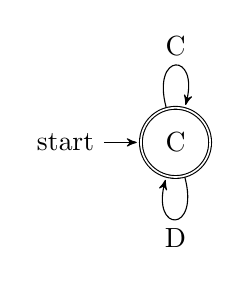
\begin{tikzpicture}[>=stealth',shorten >=1pt,auto,node distance=1cm]
\node[initial,state,accepting] (C)	{C};
\path[->] (C) edge [loop above] node {C} (C)
	edge [loop below] node {D} (C);
\end{tikzpicture}
}\hfill
\subfloat[ALLD]{\label{fig:fsa.alld}
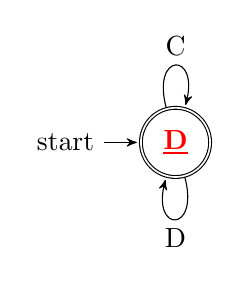
\begin{tikzpicture}[>=stealth',shorten >=1pt,auto,node distance=1cm]
\node[initial,state,accepting] (C)	{\textcolor{red}{\underline{\textbf{D}}}};
\path[->] (C) edge [loop above] node {C} (C)
	edge [loop below] node {D} (C);
\end{tikzpicture}
}\hfill
\subfloat[STFT]{\label{fig:fsa.stft}
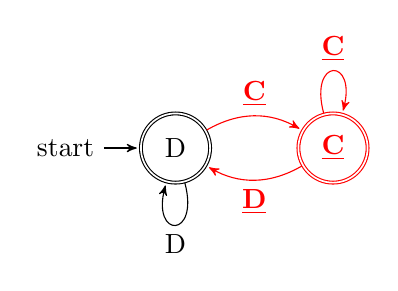
\begin{tikzpicture}[>=stealth',shorten >=1pt,auto,node distance=2cm]
\node[initial,state,accepting] (D)	{D};
\node[red, state,accepting] (C) [right of=D] {\underline{\textbf{C}}};
\path[->] (D) edge [red, bend left] node {\underline{\textbf{C}}} (C);
\path[->] (D) edge [loop below] node {D} (C);
\path[->] (C) edge [red, loop above] node {\underline{\textbf{C}}} (C);
\path[->] (C) edge [red, bend left] node {\underline{\textbf{D}}} (D);
\end{tikzpicture}
}\hfill
\caption{Finite State Automata representations of some strategies, choosing to defect or cooperate based on label of final state. Red and underlined states or transitions indicate changes needed to go from ALLC to ALLD, then ALLD to STFT.}
\label{fig:fsa}
\end{figure}

The strategy space (set of strategies) representable by a method is not the only important factor. 
The distance in strategy space between strategies can be defined as the number of mutations needed to turn one strategy into another. 
A possible mutation method for the binary string would be to flip a digit. 
In the case off ALLD and STFT, the distance is one. Flipping the second digit turns one into the other. 
The distance between the Finite State Automata representations is larger. 
The actual distance will depend on how mutations are performed. 
A state needs to be added to turn ALLD into STFT, 2 transitions added, and 1 transition moved (Figure \ref{fig:fsa}). 
To turn STFT into ALLD, a specific node is removed- the cooperate node- 2 transitions are removed, and 1 transition is moved. 
The implication of this example is that the 'topology' of the strategy space depends on representation. 
The path for evolution of a strategy differs based on this topology. 
If mutations are single flips on a string, the strategies exist on the corners of an n-dimensional hypercube where n is the length of the string. 
Adding another mechanism, such as flip all bits, changes the topology since opposite corners now have a new path to each other of length one.

Another example of this differing topology is the conversion of ALLD to ALLC and vice versa. 
In this example the mutation method for the Finite State Automaton is obvious; the outcome of the single node is flipped. 
The distance between strategies is one node flip. 
If the mutation method for the binary representation is to flip a bit, that is the flipping of all bits at once is excluded as a method, the distance in this strategy space is 3. 
Representation and mutation method both have important implications.

The history of moves consists of a sequence of options, cooperate (C) or defect (D). 
A strategy can be considered a formal language. 
Cooperation occurs when the history belongs to the language. 
Figure \ref{fig:fsa.lang} shows the Finite State Automata approach to this. 
Finite State Automata, the representation used in \citet{van-veelen:PNAS:2012}, allows only regular languages, which restricts the strategy space. 
To make the problem tractable, some representation that only represents a subset of possible strategies is required. 
Each representation for strategies has limitations, advantages and disadvantages, such as the set of strategies that can be simulated and complexity of mutation. 
In this project, non-regular strategies will be simulated.

The methodology from \citet{van-veelen:PNAS:2012} will be followed with this new representation, and how non-regular strategies effect the results examined.

\begin{figure}[h]
\subfloat[ALLC]{\label{fig:fsa.allc.lang}
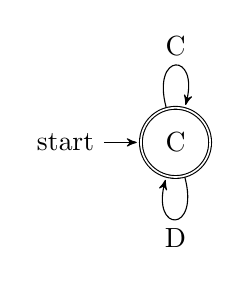
\begin{tikzpicture}[>=stealth',shorten >=1pt,auto,node distance=1cm]
\node[initial,state,accepting] (C)	{C};
\path[->] (C) edge [loop above] node {C} (C)
	edge [loop below] node {D} (C);
\end{tikzpicture}
}\hfill
\subfloat[ALLD]{\label{fig:fsa.alld.lang}
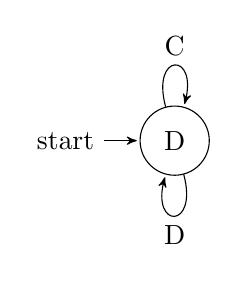
\begin{tikzpicture}[>=stealth',shorten >=1pt,auto,node distance=1cm]
\node[initial,state] (C)	{D};
\path[->] (C) edge [loop above] node {C} (C)
	edge [loop below] node {D} (C);
\end{tikzpicture}
}\hfill
\subfloat[STFT]{\label{fig:fsa.stft.lang}
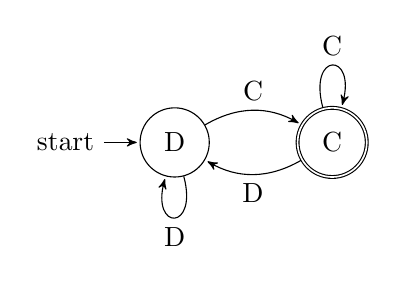
\begin{tikzpicture}[>=stealth',shorten >=1pt,auto,node distance=2cm]
\node[initial,state] (D)	{D};
\node[state,accepting] (C) [right of=D] {C};
\path[->] (D) edge [bend left] node {C} (C);
\path[->] (D) edge [loop below] node {D} (C);
\path[->] (C) edge [loop above] node {C} (C);
\path[->] (C) edge [bend left] node {D} (D);
\end{tikzpicture}
}\hfill
\caption{Finite State Automata that define languages that histories of Prisoner's Dilemma games can belong to (resulting in a choice to cooperate) or not (defect)}
\label{fig:fsa.lang}
\end{figure}
%\pagebreak[4]
\section{Research Plan and Methods}
The first task for the project is to investigate and evaluate the different possible representations for the strategies. 
This will require study of existing literature, and prototyping possible representations. 
Once a set of representations to investigate is chosen, a simulation needs to be created. 
Appropriate analysis of the simulations will check if and when results match the original simulation with finite state automaton representation for strategies. 
Based on the results of this analysis, further extensions to the research will be investigated such as the complexity of strategies as computational power is increased.

Table \ref{tbl:timetable} gives an overview of the required tasks and deadlines. 
The process will be an iterative one, for example with analysis providing ideas to investigate a modified representation. 
As such, dates serve as a guideline for these tasks to be accomplished, but not necessarily matching the final product.
\begin{table}[0.5\textwidth]
\centering
\captionsetup{justification=centering}
\begin{tabular}{|l|l|l|}
\hline
Task & Start Date & End Date\\
\hline
Research Proposal (Draft) &  7 Mar & 4 Apr\\
\hline
Research Proposal & 7 Mar &11 Apr \\
\hline
Literature Review (Draft) & 11 Apr &30 May\\
\hline
Literature Review & 30 May & 13 Jun\\
\hline
Interim Presentation & 30 May &9 Jun\\
\hline
Investigate Representations & 11 Apr & 27 Jun \\
\hline
Prototype Representations & 13 Jun & 4 Jul\\
\hline
Program Simulation & 13 Jun & 15 Jul \\
\hline
Analysis & 15 Jul  & 19 Sep\\
\hline
Final Presentation & 31 Oct & 10 Nov\\
\hline
Thesis Draft & 13 Jun & 31 Oct\\
\hline
Thesis for Examination &31 Oct & 14 Nov\\
\hline
\end{tabular}
\caption{Project Timetable}
\label{tbl:timetable}
\end{table}
%\pagebreak[4]
\subsection{Selecting Representations}
Adding computational power to agents could be accomplished by using Deterministic Push-Down Automata (DPDA), allowing the exploration of a strategy space including all strategies representable by Deterministic Context-Free Languages. 
Whilst I cannot predict what strategies will evolve, I can give examples of what strategies could evolve that could not in a regular strategy space. 
One example is making a decision based not on the exact sequence of moves, but on the ratio of moves. 
A pushdown automaton can check if the opponent has been overwhelmingly uncooperative (say, defecting 3/4 of the time) and pursue a different strategy based on this assessment. 
Since regular languages are a subset of Deterministic Context-Free Languages \citep{Sipser2006}, a pushdown automata can represent all strategies used in \citet{van-veelen:PNAS:2012}. 

The DPDA is by no means the only representation that could be selected, but highlights the task the of selecting a representation. 
More computationally powerful methods could also be used. 
These would have associated advantages like allowing a larger strategy space. 
Disadvantages include the possibility of infinite loops developing in strategies.

In this project, selecting a representation to use is the first task that must be completed. 
This will be performed in conjunction with the literature review; previous approaches to this problem in the literature will inform the decision. 
The decision process will also include prototyping each representation and examining the feasibility of using it in simulations.
%\pagebreak[1]
\subsection{Simulation}
A simulation will be created in Java, using an agent based model, based on \citet{van-veelen:PNAS:2012}. 
Test driven development methodology will be used, using JUNIT for unit tests. 
The simulation will consist of representations for strategies, a Wright-Fisher mutation process for representations, a Prisoner's Dilemma game and a selection process based on performance in the Prisoner's Dilemma. External libraries will be evaluated early in the design of the the simulation for possible use. 
Factors such as extensibility for further research such as using a different mutation process, representation or basis for structure will be considered. 

A process of stochastic mutation and selection will evolve strategies. 
To investigate the relation between structure, direct reciprocity and cooperation, assortment of the population and continuation probability will be variable. 
Simulations will be designed with best practices for scientific computing in mind \citep{wilson2014best}. 
For analysis, information such as strategies that appear in the simulation, their frequency and how long they remain in the population will be recorded. %Not reproducibility of research, thats a different thing
%\pagebreak[1]
\subsection{Analysis}
The results of the simulation will be examined, discovering the variety of strategies that evolve. 
Evolution paths, mechanisms by which strategies become a fixture in the population (such as direct invasion and indirect invasion), and cycles in the simulation between dominant strategies may be examined. 
This includes patterns such as strategies invading another strategy directly (beating it directly) and indirectly (becoming fitter than a strategy by performing better against the general population). 
For example indirect invasions display interesting cycles, where the invader does not excel until an exploitable strategy becomes sufficiently frequent in the population \citep{van-veelen:PNAS:2012}. 

This will involve some work using game theory to analyse strategies, as well as analysis of the results of the simulation. 
In particular the relation between the structure of the population, the reciprocity of the population, and the resulting cooperativity will be examined. 
%\pagebreak[4]
\section{Deliverables}
In this project an agent based simulation of evolution useful for exploring the relation between reciprocity and population structure will be produced. 
The simulation will extend the work of \citet{van-veelen:PNAS:2012}, using more computationally powerful representations for strategies. 
Software produced will consist of a simulation written in Java, unit tests for all aspects of the simulation, and technical documentation. 
It is intended the source code for this simulation will be made publicly available at the end of the project, and be part of the scientific contribution for this project. 
An analysis of the results of this simulation in the context of conclusions from previous research and game theory will also be completed. 

\bibliographystyle{dcu}
\bibliography{../bibliography}

\end{document}
